\documentclass[12pt,letterpaper]{article}

\usepackage[utf8]{inputenc}
\usepackage[T1]{fontenc}
\usepackage{amsmath}
\usepackage{amsfonts}
\usepackage{amssymb}
\usepackage{amsthm}
\usepackage[left=2cm,right=2cm,top=2cm,bottom=2cm,headheight=22pt]{geometry}
\usepackage{fancyhdr}
\usepackage{setspace}
\usepackage{lastpage}
\usepackage{graphicx}
\usepackage{caption}
\usepackage{wrapfig}


\theoremstyle{definition}
\newtheorem{question}{Question}
\newtheorem{example}{Example}
\newtheorem{exercise}[question]{Exercise}
\newtheorem*{challenge}{Challenge}

\begin{document}

%Paramètres de mise en forme des paragraphes selon les normes françaises
\setlength{\parskip}{1ex plus 0.5ex minus 0.2ex}
\setlength{\parindent}{0pt}

%Paramètres relatifs aux en-têtes et pieds de page.
\pagestyle{fancy}
\lhead{Theron J Hitchman}
\chead{\Large Meeting 13}
\rhead{Fall 2013}
\lfoot{\emph{Math and Decision Making}}
\cfoot{}
\rfoot{\emph{\thepage\ of \pageref{LastPage}}}


\begin{wrapfigure}{l}{.3\textwidth}
    \centering
    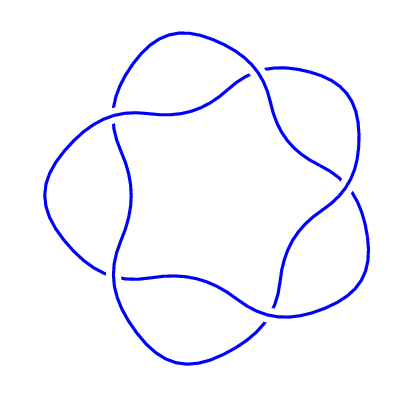
\includegraphics[width=.3\textwidth]{knotpics/5_1.png}
    \caption{The knot $5_1$}
\end{wrapfigure}
This is the knot $5_1$. Our first goal today is to compute its unknotting number $u(5_1)$.
\begin{enumerate}
\item Pick any one crossing and change it.
What knot do you get?
You might have to do a little bit of isotopy and a Reidemeister move or two before you recognize it.

\item Why is it enough to check just one crossing to show that $u(5_1) \neq 1$?

\item Find a set of two crossings so that changing those crossings transforms $5_1$ into the unknot. 
Again, after changing the crossings, you might have to move things around a bit.
\end{enumerate}



\clearpage


\begin{wrapfigure}{l}{.3\textwidth}
    \centering
    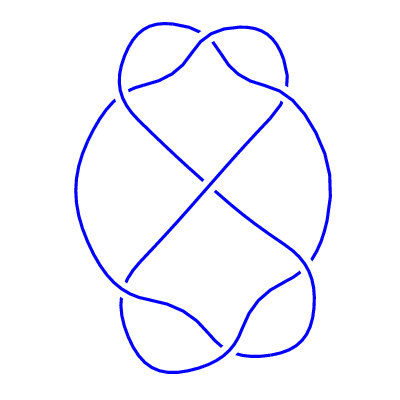
\includegraphics[width=.3\textwidth]{knotpics/7_4.png}
    \caption{The knot $7_4$.}
\end{wrapfigure}
This is the knot $7_4$. 
You may recall that you proved $7_4$ is tricolorable in a Reading and Guided Practice assingment.
Our next goal is to figure out the unknotting number of this knot, $u(7_4)$.
\begin{enumerate}
\item Consider the case of a single crossing change.
For six of the crossings, if you just change that single crossing you should get the same resulting knot.
It might take a little bit of moving things around.
What knot is that?
(Hint: You saw it in Reading and Guided Practice 12.)

\item For the seventh crossing, changing just that one crossing produces another, more familiar knot. 
Which one is it?

\item Is that enough information to show that $u(7_4) \neq 1$?

\item Find a set of two crossings so that changing those crossings transforms $7_4$ into the unknot.
\end{enumerate}

\end{document}
%sagemathcloud={"zoom_width":100}